\documentclass[a4paper,11pt]{article}

\usepackage[italian]{babel}
\usepackage[utf8]{inputenc} % permette l'inserimento di caratteri accentati da tastiera nel documento sorgente.
\usepackage[T1]{fontenc} % specifica la codifica dei font da usare nel documento stampato.
\usepackage{times} % per caricare un font scalabile
\usepackage{graphicx}
\usepackage{placeins}


\begin{document}

\textbf{Design Pattern}

\tableofcontents %indice
\listoffigures
\pagebreak

\section{Strutturali}
Affrontano i problemi che riguardano la composizione di classi e oggetti, consentendo il riutilizzo di oggetti esistenti, sfruttando l’ereditarietà e l’aggregazione.

\subsection{Adapter}
Viene utilizzato per cambiare l’interfaccia di una classe in un’altra, in modo da poter inserire all’interno delle gerarchi dell’applicazione classi già esistenti o componenti di toolkit.

\begin{figure}[ht]
    \centering
    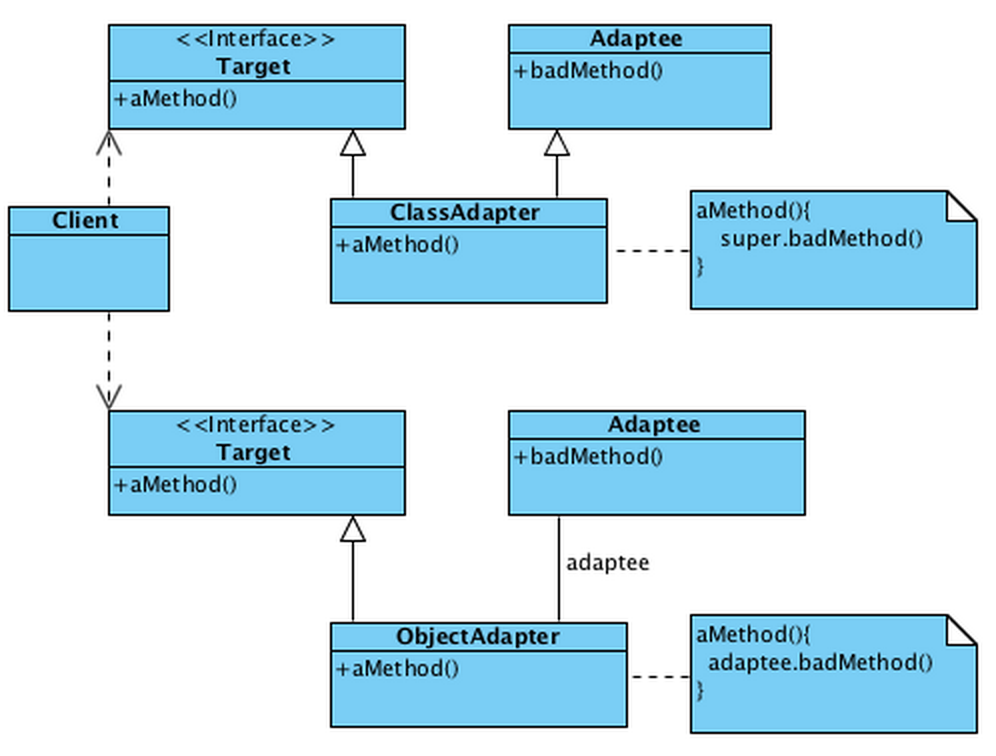
\includegraphics[width=0.8\textwidth]{immagini/adapter.png}
    \caption{Adapter}
\end{figure}
\FloatBarrier

Può essere realizzato in due modi distinti:
\begin{itemize}
\item \textbf{Class Adapter:} in cui la classe Adapter implementa sia l’interfaccia della classe da adattare (Adaptee) sia l’interfaccia Target. Questa modalità non funziona quando bisogna adattare una classe e anche le sue sottoclassi, però permette all’Adapter di modificare alcune caratteristiche dell’Adaptee.
\item \textbf{Object Adapter:} in cui la classe Adapter implementa solamente l’interfaccia Target e utilizza un’oggetto di tipo Adaptee sul quale esegue le azioni. Questa modialità permette ad Adapter di funzionare sia con Adaptee sia con le sue sottoclassi, tuttavia non è possibile modificare l’oggetto Adaptee.
\end{itemize}
In ogni caso un oggetto di tipo Adapter non è sottotipo di Adaptee.
\subsection{Decorator}
Viene utilizzato per aggiungere funzionalità ad un oggetto dinamicamente, senza usare il subclassing.
Si vuole \textit{"wrappare”} un componente dentro un decoratore per aggiungergli delle funzionalità. Per rendere più potente il tutto, sfruttando un’interfaccia comune è possibile decorare un decoratore e così via.
Al livello implementativo il Component dovrebbe essere stateless e le modifiche apportate dal Decorator dovrebbero essere leggere, in altri casi conviene usare il pattern Strategy, in modo da evitare decoratori costosi da manutenere.

\begin{figure}[ht]
    \centering
    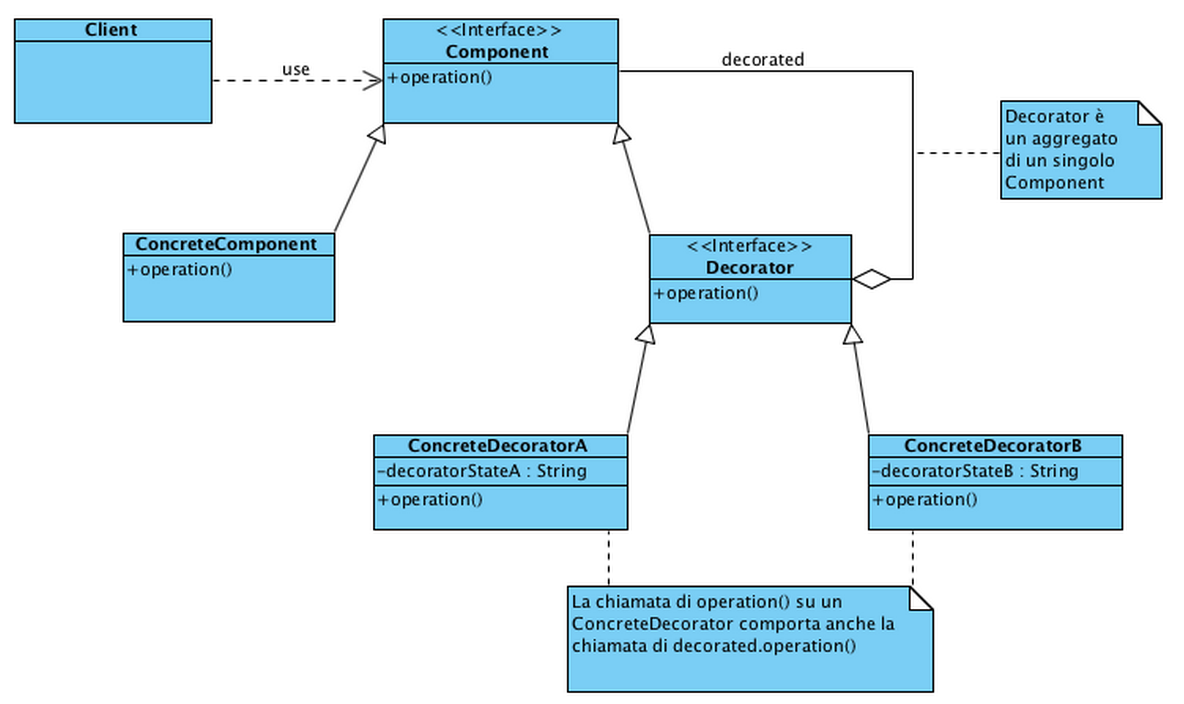
\includegraphics[width=0.8\textwidth]{immagini/decorator.png}
    \caption{Decorator}
\end{figure}
\FloatBarrier
\subsubsection{Utilizzo}
Prima creo il ConcreteComponent, poi usando creo i vari Decoratori, passandogli come riferimento il compoente: \\
\texttt{Component c = new ConcreteDecoratorB(new ConcreteDecoratorA(new ConcreteComponent));}

\subsection{Facade}
Viene usato per fornire un’interfaccia unica e semplice per un sotto sistema complesso.
In questo modo vengono semplificate le varie dipendenze tra i sotto sistemi, senza nascondere le funzionalità di basso livello.
Di conseguenza:
\begin{itemize}
\item Diminuiscono le classi del sotto sistema con il quale il client deve interagire;
\item C’è un accoppiamento lasco tra i sotto sistemi, senza dipendeze circolari;
\item Viene introdotto un single point of failure;
\item \`{E} necessario prestare attenzione al dimensionamento della classe Facace che non deve essere troppo grande.
\end{itemize}
\begin{figure}[ht]
    \centering
    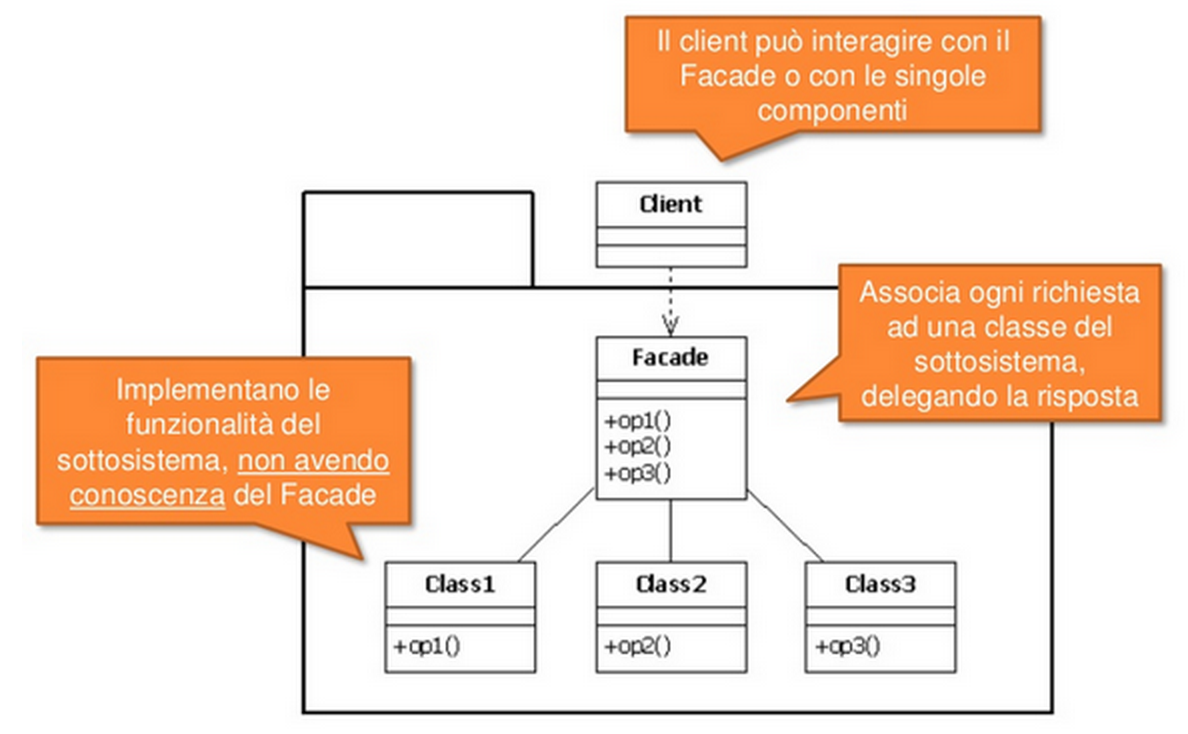
\includegraphics[width=0.8\textwidth]{immagini/facade.png}
    \caption{Facade}
\end{figure}
\FloatBarrier
\subsection{Proxy}
Viene utilizzato per fornire un surrogato di un altro oggetto di cui si vuole controllare l’accesso. Questo surrogato deve quindi agire come l’oggetto che rappresenta e perciò devono condividere la stessa interfaccia.
Questo pattern ha diversi utilizzi pratici:
\begin{itemize}
\item \textbf{Remote proxy}: rappresentazione locale di un oggetto remoto (JavaRMI)
\item \textbf{Virtual proxy}: creazione ritardata di oggetti (Lazy instantiation)
\item \textbf{Protection proxy}: controllo degli accessi all’oggetto originale
\item \textbf{Puntatore intelligente}: per una gestione efficace della memoria (Copy on edit)
\end{itemize}
\begin{figure}[ht]
    \centering
    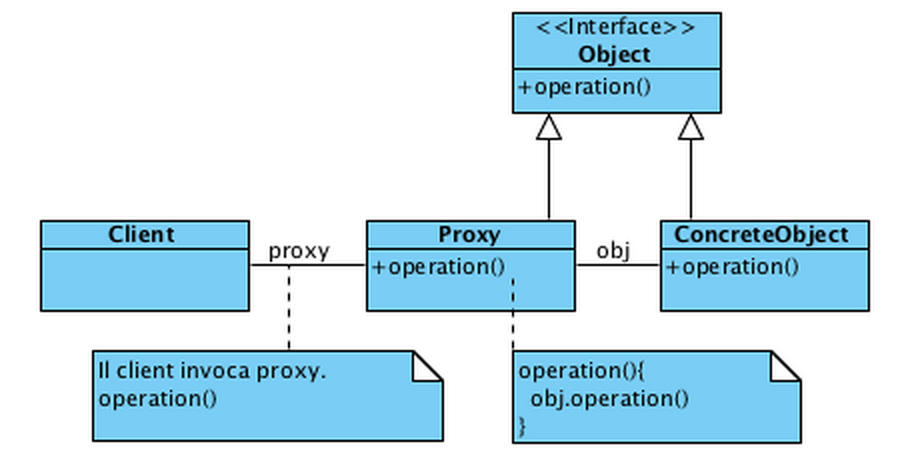
\includegraphics[width=0.8\textwidth]{immagini/proxy.png}
    \caption{Proxy}
\end{figure}
\FloatBarrier

%\subsection{Composite}
Probabilmente non è stato affrontato da Cardin % Non affrontato

\section{Creazionali}
Lo scopo di questa serie di design pattern è quello di rendere un sistema indipendente dall'implementazione delle sue compoenti, nasconendo i tipi concreti mediante l'utilizzo di inferfacce e classi astratte.
\subsection{Singleton}
Viene utilizzato quando si vuole assicurare l'esistenza di un'unica istanza di una determinata classe e si vuole fornire un unico punto d'accesso globale a questa istanza.
\begin{figure}[ht]
    \centering
    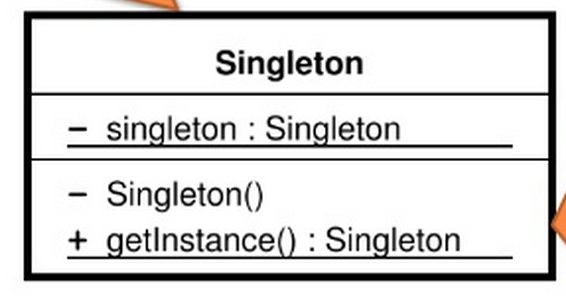
\includegraphics[width=0.8\textwidth]{immagini/singleton.png}
    \caption{Singleton}
\end{figure}
\FloatBarrier
La classe viene quindi definita con un costruttore privato e l'unico modo per crearla è tramite un metodo pubblico, che, controlla se esiste già un'istanza e nel caso esista, ritorna un riferimeto a quell'istanza anziché creare un nuovo oggetto.
Utilizzando questo pattern si riesce ad avere un controllo completo sul numero di istanze presenti e sul come i vari client possono accedervi, evitando l'utilizzo di variabili globali e rendendo possibile applicare anche il polimorfismo.
\subsection{Builder}
Viene utilizzato per separare la logica di costruzione di un oggetto complesso dalla sua rappresentazione. Permette inoltre di creare dinamicamente dei nuovi oggetti mediante degli algoritmi di creazione che sono facilmente intercambiabili tra loro.

\begin{figure}[ht]
    \centering
    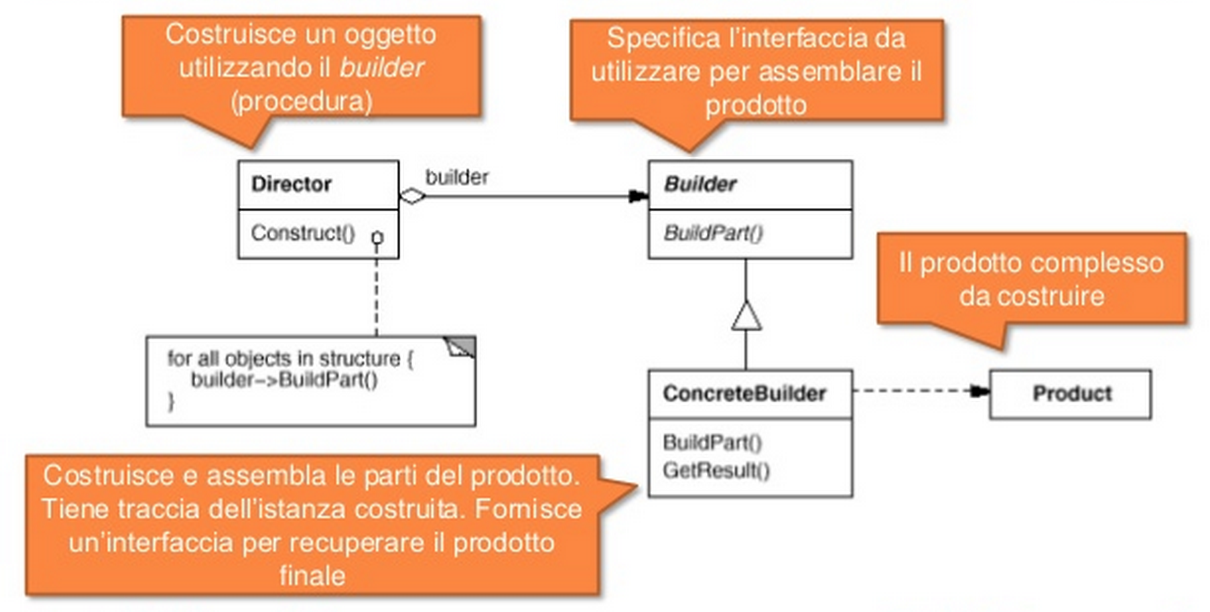
\includegraphics[width=0.8\textwidth]{immagini/builder.png}
    \caption{Builder}
\end{figure}
\FloatBarrier

In questo modo viene isolato il codice di costruzione dell'oggetto, rendendolo più facile da estendere senza far esplodere il numero di parametri da passare al costruttore (telescoping).
Inoltre, se vengono aggiunti campi, non è necessario andare a modificare il codice del client, ma le modifiche vengono limitate al director.
\subsubsection{Utilizzo}
\begin{enumerate}
\item Il client crea un builder per l'oggetto che deve costruire;
\item Il client crea un director passandogli il builder con cui costruire l'oggetto;
\item Il director crea l'oggetto finale utilizzando i vari metodi messi a disposizione dal builder;
\item Il client ottiene il riferimento all'oggetto finale.
\end{enumerate}
\begin{figure}[ht]
    \centering
    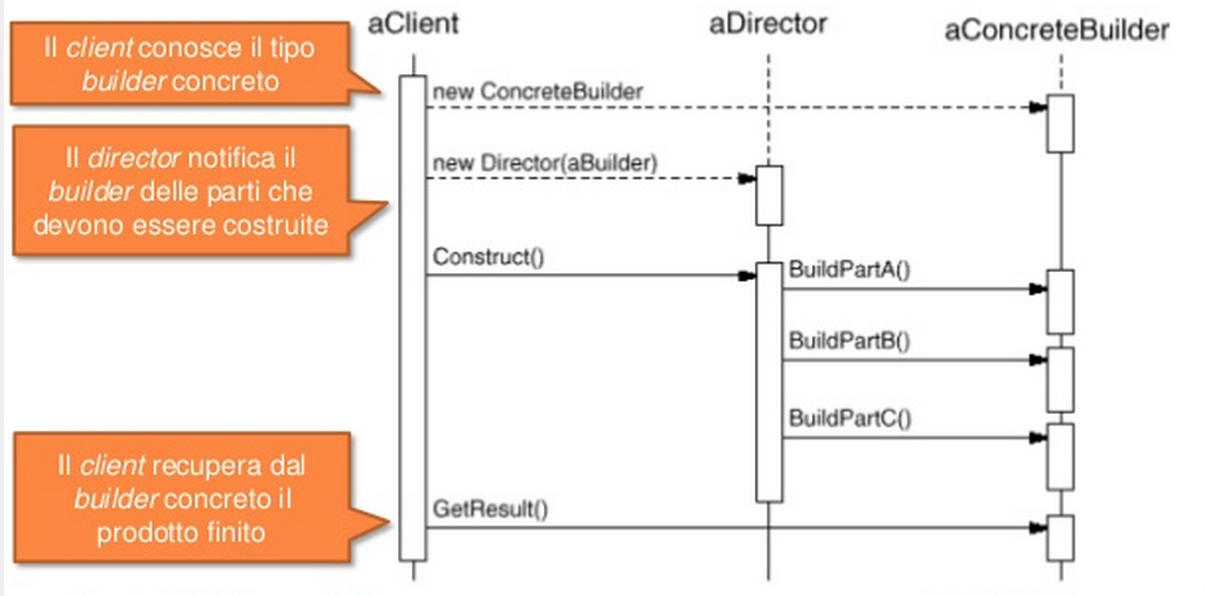
\includegraphics[width=0.8\textwidth]{immagini/builderSequence.png}
    \caption{Diagramma di sequenza di un builder}
\end{figure}
\FloatBarrier

\subsection{Abstract Factory}
Viene utilizzato per fornire la possibilità al client di creare oggetti appartenenti ad una gerarchia di prodotti, senza dover specificare le classi concrete.
\begin{figure}[ht]
    \centering
    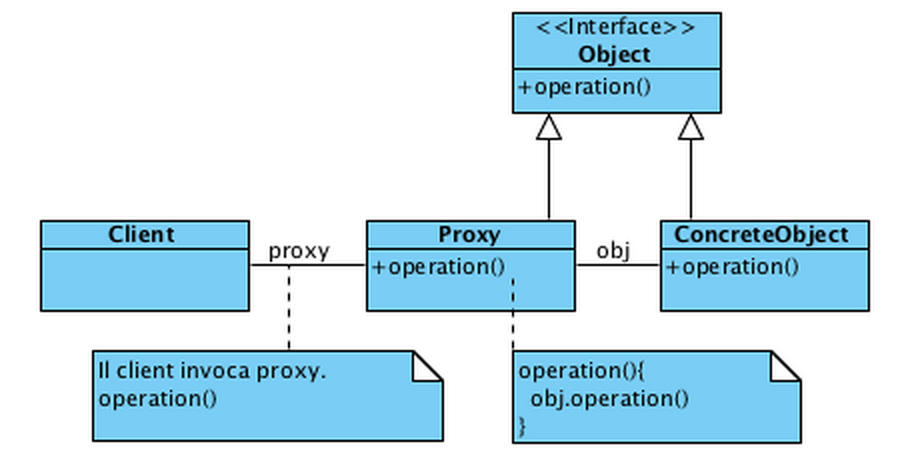
\includegraphics[width=0.8\textwidth]{immagini/proxy.png}
    \caption{Proxy}
\end{figure}
\FloatBarrier

Utilizzando questo pattern le classi client possono lavorare semplicemente con le interfacce, senza aver bisogno di conoscere i tipi concreti.
Tendenzialmente una Abstract Factory implementa un Singleton.

\subsubsection{Casi tipici}
\begin{itemize}
\item La creazione di oggetti deve essere indipendente dal sistema che li utilizza;
\item Il sistema deve poter lavorare con più famiglie degli stessi oggetti;
\item Varie famiglie di oggetti devono essere usate assieme;
\item Devono essere pubblicate delle librerie e non si vogliono mostrare i dettagli implementativi;
\item Il client non deve conoscere le classi concrete con cui lavora.
\end{itemize}
%\subsection{Factory Method}
Non affrontato da Cardin % Non affrontato


\section{Comportamentali}
Lo scopo di questa serie di design pattern è quello di poter definire dinamicamente come degli oggetti collaborano tra loro e come svolgono la loro funzione.

\subsection{Command}
Viene utilizzato per incapsulare delle richieste all'interno di un oggetto, in modo che il client siano indipendenti dal tipo di richiesta.

\begin{figure}[ht]
    \centering
    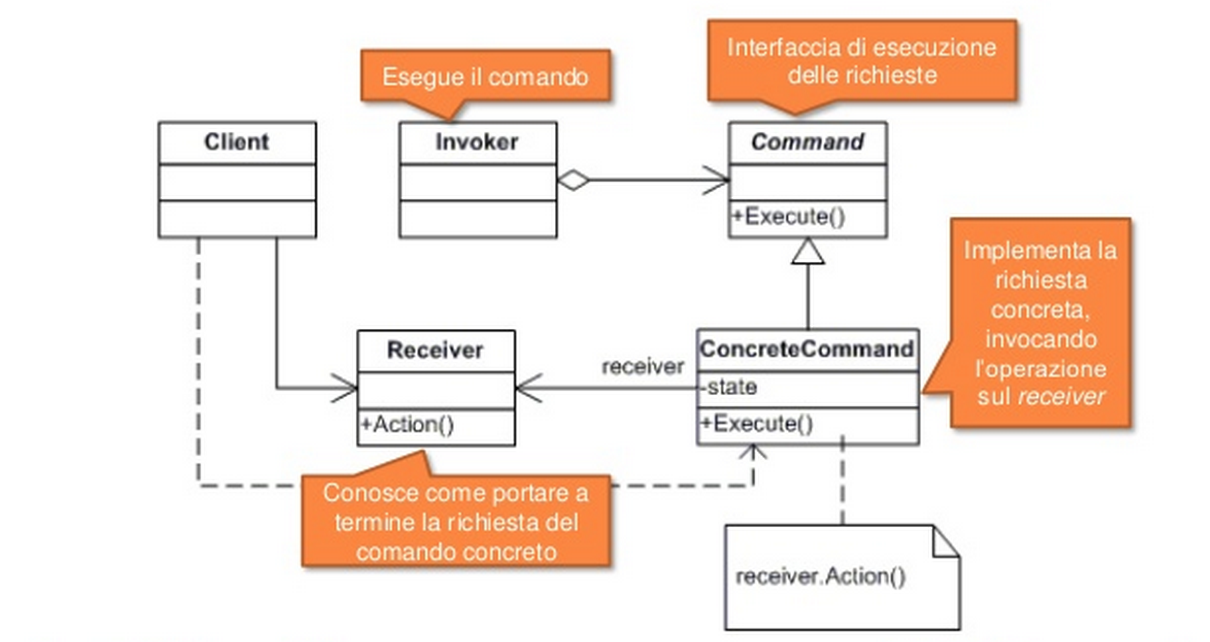
\includegraphics[width=0.8\textwidth]{immagini/command.png}
    \caption{Command}
\end{figure}
\FloatBarrier

\subsubsection{Utilizzo}
\begin{enumerate}
\item Il client crea il comando da eseguire;
\item Il client passa il comando da eseguire all'invoker (oggetto che si occupa di gestire i comandi);
\item L'invoker eseguire il comando, producendo degli effetti sul reciver.
\end{enumerate}
\begin{figure}[ht]
    \centering
    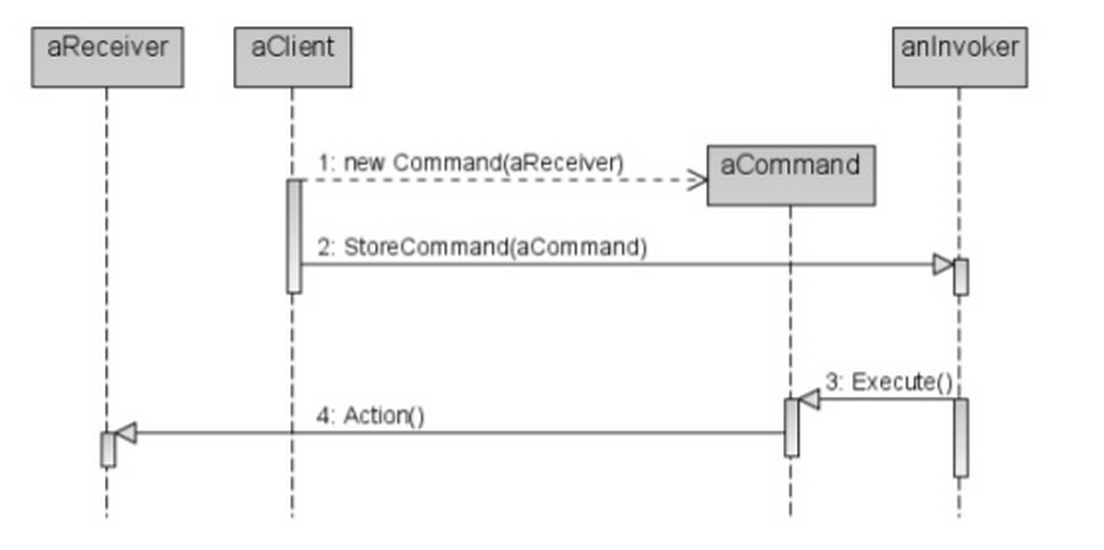
\includegraphics[width=0.8\textwidth]{immagini/commandSequence.png}
    \caption{Diagramma di sequenza - Command pattern}
\end{figure}
\FloatBarrier


\subsubsection{Casi tipici}
\begin{itemize}
\item Sono necessarie delle funzionalità di callback;
\item Le richieste devono essere gestite in momenti differenti o in ordine diverso;
\item \`{E} necessario tenere uno storico delle richieste effettuate;
\item Tra il chiamante e il ricevente deve esserci un accoppiamento lasco.
\end{itemize}
\subsection{Iterator}
Viene utilizzato per permette ad una classe client di effettuare l'accesso sequenziale agli elementi di un aggregato, senza esporre l'implementazione dell'oggetto.

\begin{figure}[ht]
    \centering
    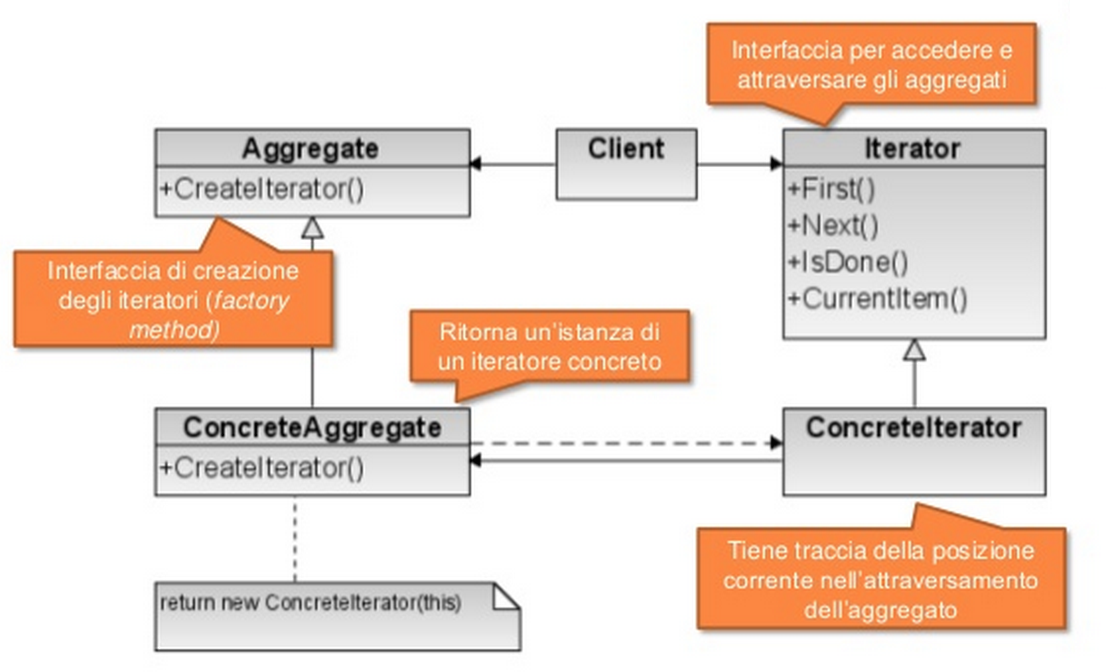
\includegraphics[width=0.8\textwidth]{immagini/iterator.png}
    \caption{Iterator}
\end{figure}
\FloatBarrier

Nonostante il concetto di iteratore sia di per se semplice, quando viene implementato è necessario fare alcune considerazioni riguardo la logica di attraversamento e al comportamento quando vengono aggiunti o tolti dei componenti durante l'uso dell'iteratore.
Difatti, il controllo dell'iterazione può essere fatto sia dal client, invocando un metodo dell'iteratore, sia dall'iteratore stesso in modo automatico. Allo stesso modo, l'algoritmo di attraversamento può essere definito dall'aggregato oppure dall'iteratore stesso.

\subsubsection{Casi tipici}
\begin{itemize}
\item \`{E} necessario accedere agli elementi di una collezione senza sapere come sono memorizzati;
\item C'è bisogno di poter attraversare la collezione più molte, anche in modo concorrente;
\item Si vuole fornire un'inferfaccia uniforme di attraversamento;
\item Ci possono essere più modi per attraversare la stessa collezione.
\end{itemize}
\subsection{Observer}
Viene utilizzato per stabilire una relazione 1 a n tra un oggetto e altri vari oggetti che dipendo da esso.
Ogni volta che l'oggetto osservato viene modificato, questo si preoccupa di comunicarlo agli oggetti che lo osservano.

\begin{figure}[ht]
    \centering
    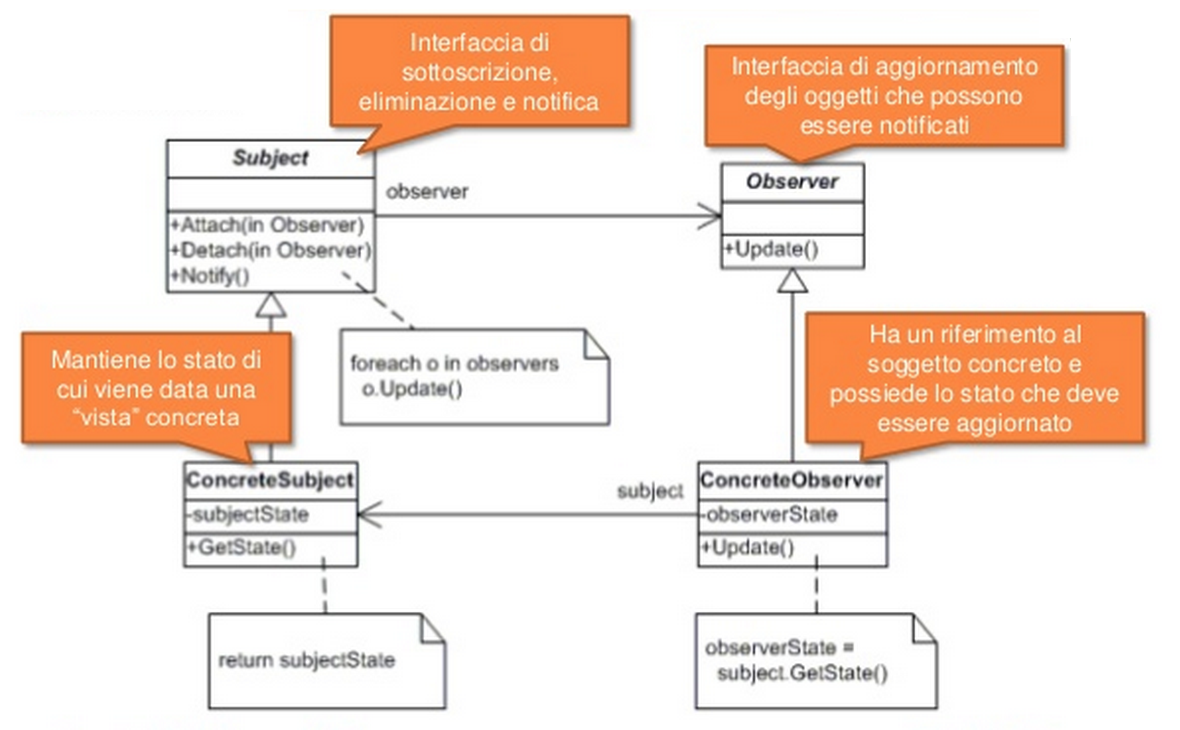
\includegraphics[width=0.8\textwidth]{immagini/observer.png}
    \caption{Proxy}
\end{figure}
\FloatBarrier

Possono essere fatte versioni più smart, dove l'oggetto osservato comunica anche che cosa è stato modificato oppure avverte solo alcuni oggetti registrati, in modo da evitare chiamate a funzioni inutili.

\subsubsection{Utilizzo}
\begin{enumerate}
\item Il soggetto viene modificato;
\item Il soggetto notifica tutti gli osservatori registrati;
\item I vari osservatori si sincronizzano sui cambiamenti subiti dal soggetto.
\end{enumerate}
\begin{figure}[ht]
    \centering
    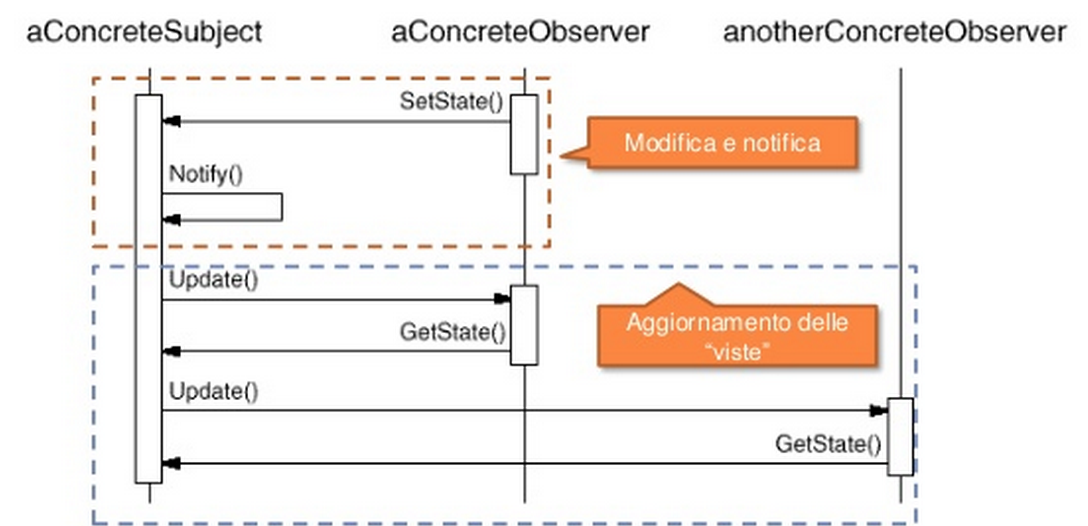
\includegraphics[width=0.8\textwidth]{immagini/observerSequence.png}
    \caption{Proxy}
\end{figure}
\FloatBarrier


\subsubsection{Casi tipici}
\begin{itemize}
\item Quando è necessario che al cambiamento di stato di un oggetto, altri oggetti eseguano delle azioni;
\item Quando è richiesto di fare il broadcast di un evento;
\item Per ottenere un accoppiamento ``astratto'' tra soggetti e osservatori.
\end{itemize}
\subsection{Strategy}
Viene utilizzato quando si ha un gruppo di algoritmi e si vuole poter scegliere l'algoritmo da adottare a runtime.
\begin{figure}[ht]
    \centering
    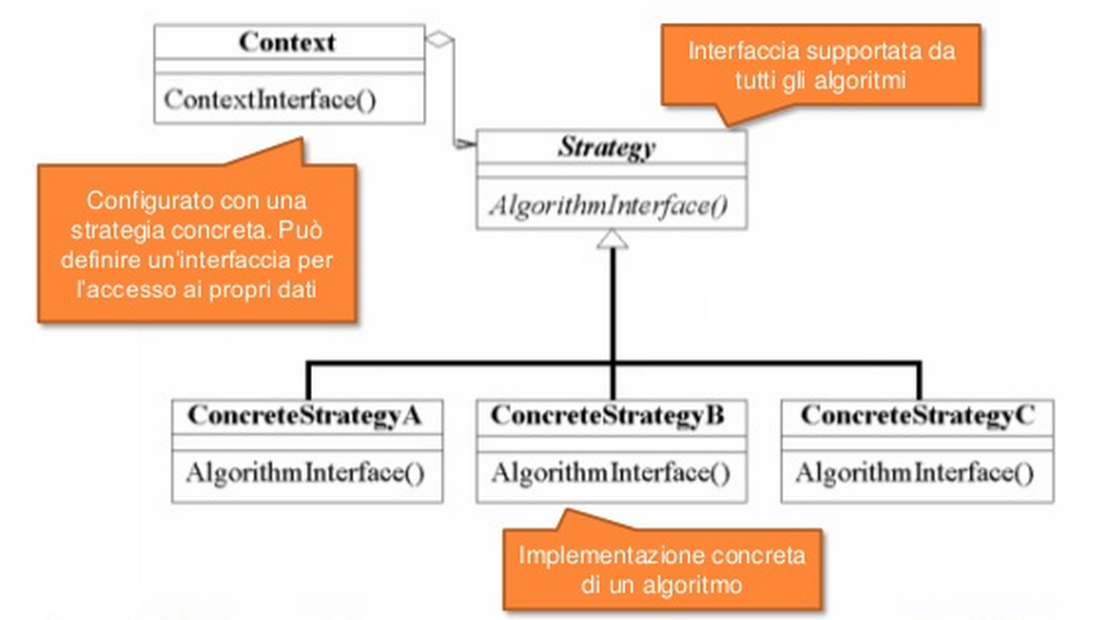
\includegraphics[width=0.8\textwidth]{immagini/strategy.png}
    \caption{Strategy}
\end{figure}
\FloatBarrier
In questo modo è anche più semplice inserire un nuovo algoritmo più efficiente, infatti, basta creare una nuova classe che lo implementa.

\subsubsection{Casi tipici}
\begin{itemize}
\item L'unica differenza tra varie classi correlate è il comportamento;
\item Sono necessarie più versioni di uno stesso algoritmo;
\item Gli algoritmi accedono o utilizzano dei dati che il codice client non deve conoscere;
\item Il comportamento di una classe deve essere definito a runtime.
\item Quando una classe definisce una serie di differenti comportamenti condizionali\footnote{Quando ci sono tanti if per scegliere l'algoritmo effettivo}.
\end{itemize}

\subsection{Template Method}
Viene utilizzato per definire un algoritmo templatizzato, fornendo una sequenza di operazioni ma senza specificare come queste vengono svolte, sarà compito delle sottoclassi definire queste operazioni.
Differisce dallo Strategy in quanto, in questo caso l'algoritmo è uno solo che deve essere implementato, mentre nello Strategy ci sono più algoritmi differenti.

\begin{figure}[ht]
    \centering
    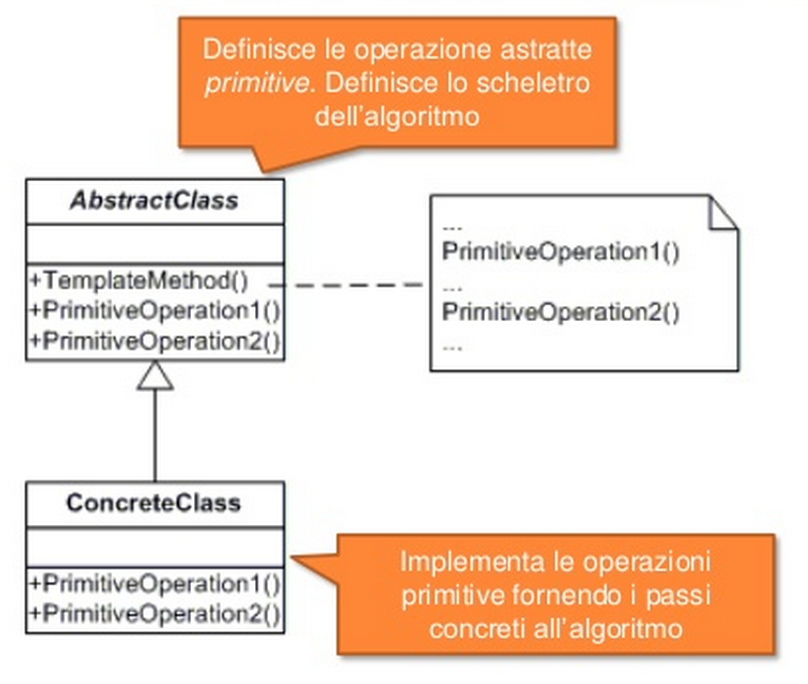
\includegraphics[width=0.8\textwidth]{immagini/templateMethod.png}
    \caption{Template method}
\end{figure}
\FloatBarrier

\subsubsection{Casi tipici}
\begin{itemize}
\item \`{E} necessaria un'unica implementazione astratta di un algoritmo;
\item Si vuole raccogliere un comportamento comune a più classi in un unica classe;
\item La classe padre deve essere in grado di eseguire i metodi delle classi figlie;
\item Tutte o quasi tutte le sottoclassi devono implementare lo stesso comportamento.
\end{itemize}
\subsection{Singleton}

\section{Architetturali}

\subsection{Dependency Injection}
Viene utilizzato per separare dalla logica di funzionamento di un componente la risoluzione delle dipendenze con gli altri oggetti.
In questo modo è possibile realizzare un \textit{inversion of control}, con un contenitore esterno che si occupa di gestire il ciclo di vita degli oggetti dell'applicazione.

Le dipendenze con gli oggetti esterni vengono quindi \textit{iniettate} dal contenitore esterno, ottenendo così una riduzione delle dipendenze e rendendo più facili i test.

La dependecy injection può essere fatta in due modi:
\begin{itemize}
\item \textbf{Constructor injection}: le dipendenze vengono iniettate passando gli oggetti come parametri del costruttore. In questo modo l'oggetto è subito utilizzabile appena viene costruito, c'è però il rischio di \textit{telescoping} sui parametri del costruttore.
\item \textbf{Setter Injection}: le dipendenze vengono iniettate passando gli oggetti mediante l'utilizzo di metodi \textit{setter}. Così viene evitato il telescoping ma per un po' di tempo dopo la creazione, l'oggetto finale rimane in uno stato inconsistente.
\end{itemize}

\subsubsection{Utilizzo}
Un sacco di framework moderni lo utilizzano:
\begin{itemize}
\item AngularJS;
\item Spring;
\item Google Guice.
\end{itemize}
\subsection{Singleton}
\end{document}